\documentclass[12pt,a4paper]{article}
\usepackage[T1]{fontenc}
\usepackage{lmodern,geometry,graphicx,xcolor,booktabs,tabularx,array,amsmath,amssymb}
\usepackage{fancyhdr,titlesec,enumitem,caption,float,microtype,listings,xurl}
\usepackage[colorlinks=true,linkcolor=navy,urlcolor=teal,citecolor=teal]{hyperref}
\geometry{left=24mm,right=24mm,top=24mm,bottom=24mm,headheight=15pt}
\definecolor{navy}{HTML}{16324F}\definecolor{teal}{HTML}{167D8D}\definecolor{light}{HTML}{EEF4F7}
\hypersetup{pdftitle={PortfolioPilot: Project Report},pdfauthor={Akhil and Ridhima},pdfsubject={Multi-objective portfolio allocation and rebalancing}}
\setlength{\emergencystretch}{3em}\setlength{\parindent}{0pt}\setlength{\parskip}{5pt}\linespread{1.04}
\titleformat{\section}{\Large\sffamily\bfseries\color{navy}}{\thesection}{0.65em}{}
\titleformat{\subsection}{\large\sffamily\bfseries\color{navy}}{\thesubsection}{0.6em}{}
\titlespacing*{\section}{0pt}{18pt}{10pt}\titlespacing*{\subsection}{0pt}{10pt}{4pt}
\setlist{itemsep=3pt,topsep=3pt,leftmargin=18pt}
\pagestyle{fancy}\fancyhf{}\fancyhead[L]{\small\sffamily\color{navy}PortfolioPilot}\fancyhead[R]{\small\sffamily Project Report}\fancyfoot[L]{\footnotesize Optimization Techniques}\fancyfoot[R]{\footnotesize\thepage}
\renewcommand{\headrulewidth}{0.4pt}\renewcommand{\footrulewidth}{0pt}
\captionsetup{font=small,labelfont=bf,skip=6pt}
\newcolumntype{Y}{>{\raggedright\arraybackslash}X}
\renewcommand{\arraystretch}{1.18}
\newcommand{\note}[1]{\par\smallskip\noindent\colorbox{light}{\parbox{\dimexpr\linewidth-2\fboxsep}{\small #1}}\par\smallskip}
\newcommand{\newsec}[1]{\section{#1}}
\lstset{basicstyle=\ttfamily\footnotesize,breaklines=true,frame=single,rulecolor=\color{light},backgroundcolor=\color{light},columns=fullflexible,keepspaces=true}
\begin{document}
\begin{titlepage}
\color{navy}\sffamily
{\small OPTIMIZATION TECHNIQUES\hfill PROJECT REPORT\par}
\vspace{20mm}
{\fontsize{38}{44}\selectfont\bfseries PortfolioPilot\par}
\vspace{5mm}
{\Large Multi-Objective Portfolio Allocation\par and Rebalancing under Return, Risk\par and Transaction-Cost Constraints\par}
\vspace{9mm}\textcolor{teal}{\rule{\linewidth}{2pt}}\par
\vspace{7mm}
{\large Evolutionary search, convex refinement\\[2mm]and evidence-based decision support\par}
\vspace{18mm}
\textbf{Submitted by}\\[5mm]
\begin{tabular}{@{}ll@{}}
Akhil & Roll No. 241070004\\[3mm]
Ridhima & Roll No. 241071062
\end{tabular}
\vfill
{\small\textbf{Project repository}\par}
\href{https://github.com/akhil-gitcoder/PortfolioPilot}{github.com/akhil-gitcoder/PortfolioPilot}\par
\vspace{6mm}
\textbf{Deployed application}\\[2mm]\href{https://portfolio-pilot-deploy.vercel.app/}{portfolio-pilot-deploy.vercel.app}
\end{titlepage}
\pagenumbering{roman}
\section*{Abstract}\addcontentsline{toc}{section}{Abstract}
Portfolio rebalancing requires an investor to balance expected return, portfolio risk and the cost of changing existing holdings. These goals conflict, while realistic limits on individual positions, sector exposure and the number of holdings make the decision space non-convex. PortfolioPilot models this problem for 30 National Stock Exchange (NSE) stocks across eight sectors and produces a set of non-dominated alternatives instead of a single prescribed portfolio.

The system implements NSGA-II from scratch using random-key encoding, constraint repair, non-dominated sorting and crowding distance. Project-specific enhancements include current-portfolio injection, sparse initialization, support-reset mutation and an external archive. The final hybrid method uses evolutionary search to choose promising stock subsets and convex optimization to refine weights on each fixed subset. Random search and a weighted-sum relax-and-round method provide comparison baselines.

Experiments use a committed snapshot of 1,729 daily price observations from January 2019 to December 2025. Across 30 random seeds, Hybrid + archive achieves mean normalized hypervolume of 0.90659, compared with 0.87705 for the deterministic weighted-sum baseline: a 3.37\% improvement. It exceeds the baseline in every run, although its recorded mean runtime is approximately 7.74 times higher. A separate rolling walk-forward evaluation over 15 quarters shows that superior estimated-front quality does not establish superior investment performance. Under the balanced selection rule, equal weight reaches final wealth of 1.8428 from unit capital, while Hybrid reaches 1.5703 and the weighted-sum method reaches 1.5641.

The project therefore demonstrates a reproducible decision-support approach for constrained multi-objective optimization, together with an explicit examination of estimation error and practical limitations. A deployed web interface presents selected alternatives, explanatory comparisons and trade amounts derived from the optimizer.

\note{\textbf{Central finding.} The hybrid method improves the quality and coverage of the estimated trade-off set. The historical evaluation does not show that it produces better realised wealth than equal weighting.}
\vspace{4mm}
\textbf{Keywords:} multi-objective optimization; NSGA-II; portfolio rebalancing; Pareto front; transaction costs; convex optimization; walk-forward evaluation.

\subsection*{Report scope and provenance}
Core implementation and recorded experiments originate from commit \texttt{482fe84}; documentation on main was inspected at \texttt{858c1b6}. The interface and deployment adapter are on \texttt{frontend}, commit \texttt{96aa4d5}. Results are taken from the committed real-data CSV and JSON outputs and checked against their generating code. Synthetic data is used for development and tests, not for the headline market results.

\clearpage\setcounter{tocdepth}{1}\tableofcontents
\clearpage\pagenumbering{arabic}
\section{Introduction and Project Objectives}
\subsection{Background and motivation}
An investor who already owns stocks must decide both what to hold next and whether the improvement justifies trading. A portfolio with a high historical average return may carry substantial volatility. A low-risk portfolio may require selling existing positions and paying transaction costs. Doing nothing incurs no immediate trading cost, but may preserve undesirable concentration.

Mean--variance portfolio selection formalizes the return--risk trade-off \cite{markowitz}. PortfolioPilot extends this setting by treating rebalancing cost as a separate objective and enforcing practical allocation rules. The investor can inspect alternative compromises rather than accept a single solution produced by an arbitrary fixed preference weight.
\subsection{Problem statement}
Given historical adjusted prices, current holdings, proportional buy/sell charges and investment constraints, identify feasible portfolios that offer useful trade-offs among:
\begin{enumerate}
\item maximizing estimated annual return;
\item minimizing annual portfolio volatility;
\item minimizing the one-off cost of moving from current to target weights.
\end{enumerate}
The starting portfolio holds six stocks. The target must remain fully invested and long-only, hold no more than ten stocks, allocate at most 20\% to one stock and at most 40\% to one sector, and assign at least 3\% to each held stock.
\subsection{Objectives and deliverables}
\begin{itemize}
\item Formulate the rebalancing problem with three explicit objectives and realistic constraints.
\item Implement a transparent evolutionary optimizer and compare it with meaningful baselines.
\item Improve search through domain-aware initialization, support exploration, archiving and convex refinement.
\item Evaluate solution quality, feasibility, repeatability and computational cost over multiple seeds.
\item Test selected portfolios on later prices with rolling estimation and trading costs.
\item Present portfolios, trades and experimental evidence through a usable interface.
\end{itemize}
\subsection{Scope}
This is an academic optimization and decision-support system. It does not execute orders, incorporate an investor's full financial circumstances or guarantee returns. Portfolio weights are continuous fractions; whole-share lot sizing, cash balances and operational execution are outside the implemented model.

\newsec{Related Work and Design Rationale}
\begin{table}[H]\centering\small
\begin{tabularx}{\linewidth}{@{}p{32mm}YY@{}}\toprule
Foundation & Relevant idea & Role in PortfolioPilot\\\midrule
Markowitz (1952) \cite{markowitz} & Expected return and covariance determine portfolio risk--return trade-offs. & Return and volatility objectives.\\
Deb et al. (2002) \cite{deb} & Elitist multi-objective search with non-dominated sorting and crowding. & NSGA-II implementation and diversity management.\\
Chang et al. (2000) \cite{chang} & Cardinality-constrained portfolio optimization introduces discrete choices. & Motivation for searching over held-stock subsets.\\
Lobo et al. (2007) \cite{lobo} & Portfolio optimization can model proportional and fixed trading costs. & Proportional buy/sell cost objective; fixed fees are excluded here.\\
Ledoit and Wolf (2004) \cite{ledoit} & Shrinkage improves covariance conditioning. & Ledoit--Wolf covariance estimator.\\
DeMiguel et al. (2009) \cite{demiguel} & Estimation error can erode the benefits of optimized portfolios. & Equal-weight benchmark and out-of-sample assessment.\\
Diamond and Boyd (2016) \cite{cvxpy} & Convex models can be expressed and solved through CVXPY. & Relaxed baseline, fixed-support polish and validation reference.\\\bottomrule
\end{tabularx}
\caption{Literature foundations and their implementation roles.}
\end{table}
\subsection{Why a hybrid approach?}
The held-stock set is a discrete choice. Once that set is fixed, weights can be optimized using a convex model. This structure suggests dividing the work: evolutionary search explores subsets, while a convex solver refines continuous allocations. Pure random search ignores search history; plain NSGA-II may discover reasonable subsets but leave their weights suboptimal. The hybrid targets both weaknesses.
\subsection{Nature of the contribution}
The project does not claim to invent NSGA-II, covariance shrinkage or convex optimization. Its contribution is their problem-specific integration with feasibility repair, a no-trade reference, support mutation, an archive, transparent comparison experiments and an explanatory interface. These are implemented engineering contributions; proposed research extensions are listed separately in Section~\ref{sec:future}.

\newsec{Data, Estimation and Assumptions}
\begin{table}[H]\centering
\begin{tabularx}{\linewidth}{@{}p{49mm}Y@{}}\toprule
Item & Dataset and configuration\\\midrule
Universe & 30 NSE stocks; eight sectors; fixed ticker list.\\
Source & Yahoo Finance adjusted closing prices via \texttt{yfinance}.\\
Committed snapshot & 1,729 price rows, 1 January 2019--30 December 2025.\\
Initial estimation window & First 756 price rows, ending 20 January 2022; 755 daily returns.\\
Remaining observations & 973 price rows; walk-forward uses 15 complete 63-day holding periods.\\
Return estimator & Arithmetic sample mean of daily simple returns, multiplied by 252.\\
Risk estimator & Ledoit--Wolf daily covariance, multiplied by 252.\\
Cost assumptions & Buy 0.00119; sell 0.00104 of traded capital.\\\bottomrule
\end{tabularx}
\caption{Data and estimation settings used for real-data results.}
\end{table}
For adjusted price $P_{t,i}$, daily simple return is $r_{t,i}=P_{t,i}/P_{t-1,i}-1$. With $T$ daily observations in the estimation window,
\[
\widehat\mu_i=252\left(\frac{1}{T}\sum_{t=1}^{T}r_{t,i}\right),\qquad
\widehat\Sigma=252\widehat\Sigma_{\mathrm{LW}}.
\]
These are estimates, not forecasts with guaranteed accuracy. The annual arithmetic mean is distinct from compound annual growth measured on a realised wealth series.
\subsection{Current portfolio and universe}
The hypothetical initial allocation is RELIANCE 20\%, TCS 20\%, HDFCBANK 20\%, ITC 15\%, SBIN 15\% and LT 10\%. It satisfies the configured limits, making no-trade a feasible zero-cost reference. Sector groups are Financials (5 stocks), IT (4), FMCG (4), Energy/Power (5), Auto (3), Pharma (3), Materials (4) and Infrastructure/Telecom (2). Appendix~\ref{app:universe} lists the complete universe.
\subsection{Data treatment and model assumptions}
The committed CSV has no missing price cells. Its fixed snapshot supports repeatable experiments even if upstream adjusted prices are revised. The download pipeline forward-fills limited gaps and drops incomplete rows; corporate-action adjustments are inherited from the provider. Synthetic factor-model data is retained only for development.

Charges are project assumptions, not independently verified live broker rates. The model excludes fixed depository/order fees, bid--ask spreads, market impact and capital-gains taxes. It assumes no leverage or short selling. A fixed, retrospectively selected stock universe may introduce selection or survivorship bias.

\newsec{Mathematical Formulation}
Let $n=30$; $x_i$ be the target weight of stock $i$; $x_i^{old}$ its current weight; $\mu$ estimated annual returns; $\Sigma$ annual covariance; and $S_k$ the stock indices in sector $k$. Buy and sell rates are $b_i$ and $s_i$.
\subsection{Three objectives}
All objectives are minimized internally:
\begin{align}
f_1(x)&=-\mu^\top x,\label{eq:return}\\
f_2(x)&=\sqrt{x^\top\Sigma x},\label{eq:risk}\\
f_3(x)&=\sum_{i=1}^{n}\left[b_i\max(x_i-x_i^{old},0)+s_i\max(x_i^{old}-x_i,0)\right].\label{eq:cost}
\end{align}
The first expression reverses return's sign for minimization. Volatility measures dispersion, not worst-case loss. Cost is a one-off fraction of capital; it is not an annual rate.
\subsection{Feasibility constraints}
A binary variable $z_i$ can describe whether stock $i$ is held:
\begin{align}
\sum_{i=1}^{n}x_i&=1, & 0.03z_i\leq x_i&\leq0.20z_i,\\
\sum_{i\in S_k}x_i&\leq0.40\quad \forall k, & \sum_{i=1}^{n}z_i&\leq10,\quad z_i\in\{0,1\}.
\end{align}
This equivalent mathematical representation makes the discrete choices explicit. The implementation uses random keys and repair rather than solving directly for binary variables. At least five positions are necessary because the single-stock cap is 20\%. The optional turnover constraint exists in code but is disabled in the reported configuration.
\subsection{Pareto optimality and problem structure}
A feasible portfolio $x$ dominates $y$ when $f_j(x)\leq f_j(y)$ for every objective and at least one inequality is strict. The approximate Pareto front contains solutions not dominated by another returned solution. It is not a certificate of global optimality.

Return is linear, volatility is convex for positive-semidefinite $\Sigma$, and proportional trading cost is convex and piecewise linear. Removing cardinality and minimum-position restrictions gives a convex feasible set. With these restrictions, selecting the support becomes combinatorial: there are $\binom{30}{10}=30{,}045{,}015$ possible ten-stock subsets before weights are considered.
\note{\textbf{Budget convention.} Target weights sum to one. The walk-forward simulator deducts cost from wealth before investing the remaining wealth at those weights. The formulation is a simplified proportional-cost model, not a detailed self-financing trade-execution model.}

\newsec{System Architecture and Implementation}
\begin{figure}[H]\centering
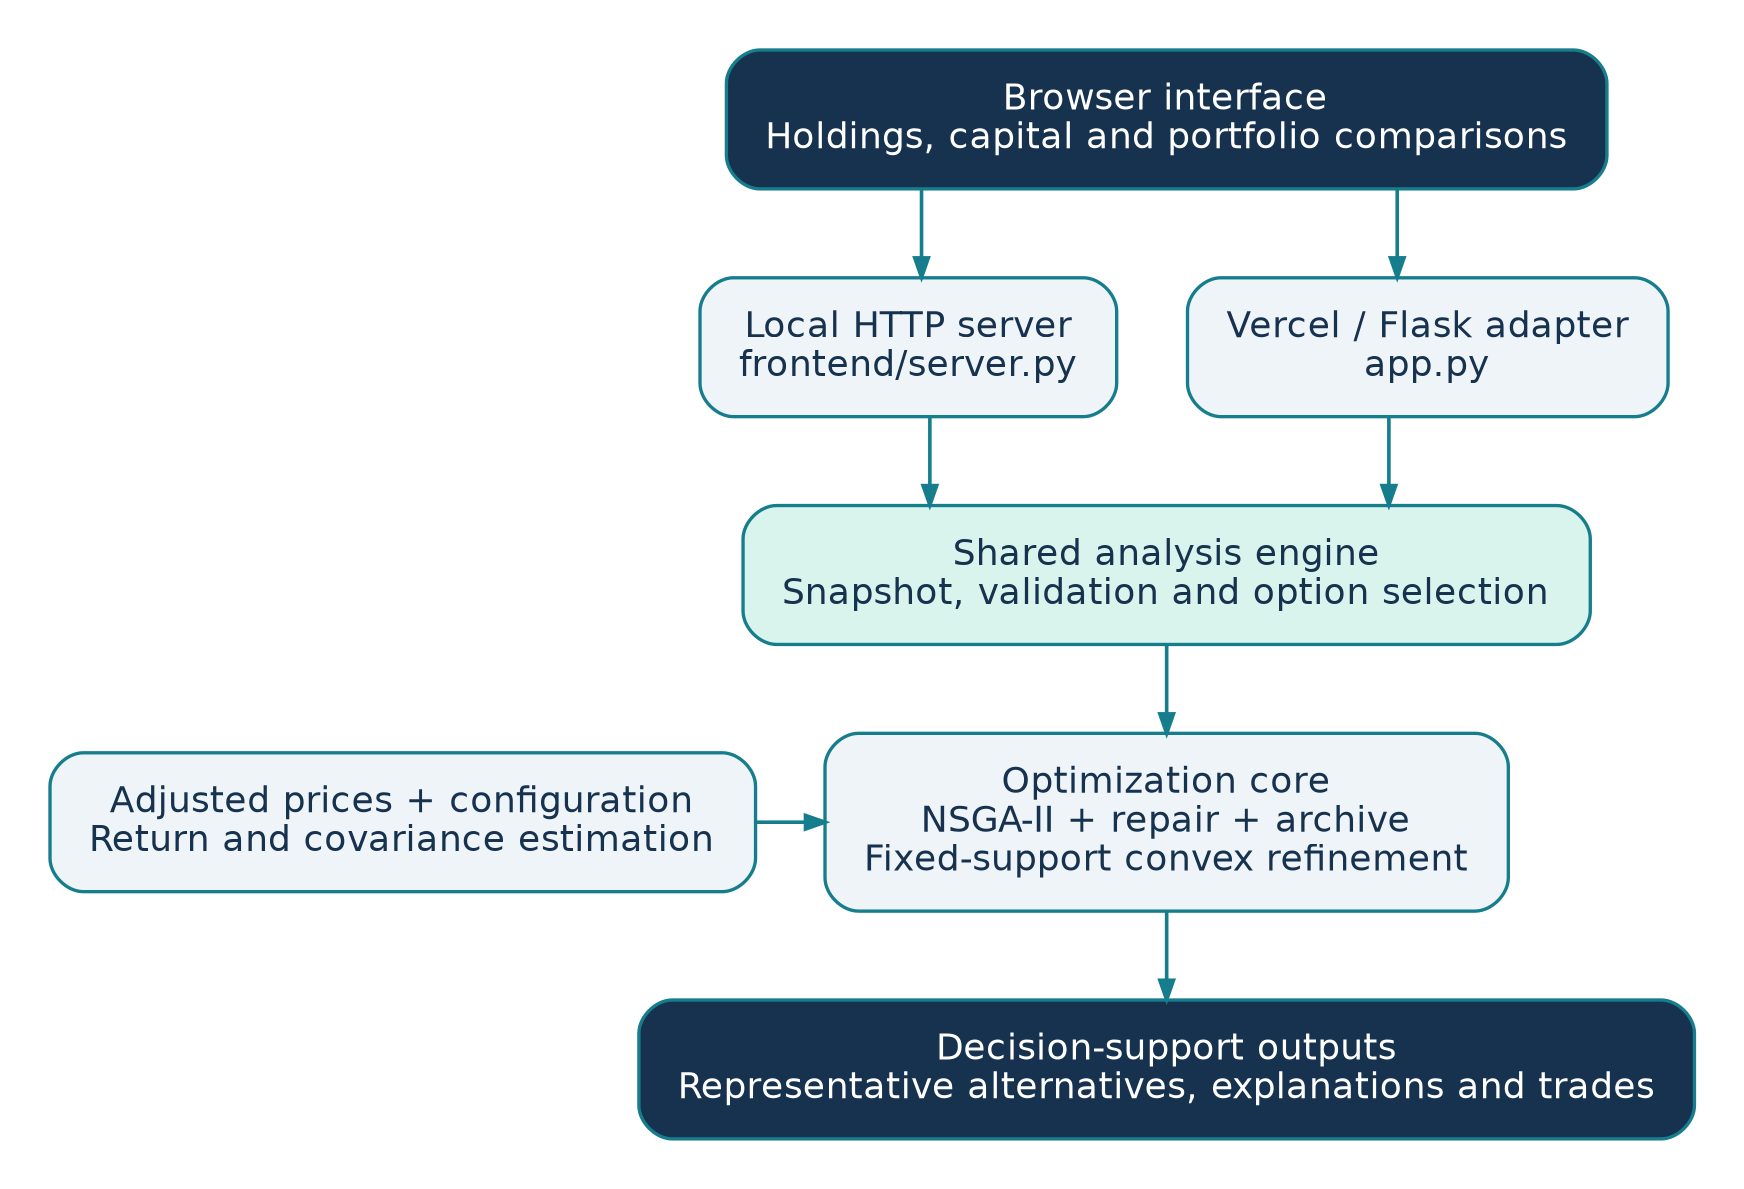
\includegraphics[width=\linewidth]{images/system_architecture.png}
\caption{System architecture linking the browser, Python API, optimization engine and recorded evidence. The local and deployed entry points share the same core engine.}
\end{figure}
\begin{table}[H]\centering\small
\begin{tabularx}{\linewidth}{@{}p{49mm}Y@{}}\toprule
Module & Responsibility\\\midrule
\texttt{src/data\_loader.py} & Read configuration and prices; estimate inputs; construct the problem.\\
\texttt{src/problem.py} & Calculate objectives, violations, support repair and weight projection.\\
\texttt{src/algorithms/nsga2.py} & Selection, variation, survivor selection and bounded archive.\\
\texttt{src/baseline/}, \texttt{src/hybrid/} & Baselines and fixed-support convex refinement.\\
\texttt{src/metrics.py}, \texttt{experiments/} & Indicators, multi-seed comparison and walk-forward orchestration.\\
\texttt{frontend/} & Browser UI, shared API logic, option selection and explanations.\\\bottomrule
\end{tabularx}
\caption{Core implementation map.}
\end{table}
Python is the implementation language. NumPy and pandas support array and data operations; SciPy supports statistical tests; scikit-learn supplies Ledoit--Wolf estimation; CVXPY with CLARABEL solves convex subproblems. Matplotlib generates charts, and pytest checks behavior. NSGA-II, repair, the archive and quality indicators are implemented in the repository rather than delegated to a multi-objective optimization framework.

\newsec{Optimization Methods}
\subsection{Random search baseline}
Generate 10,000 random-key vectors, decode each with the same repair mechanism used by NSGA-II, evaluate all objectives and retain non-dominated feasible results. This tests whether evolutionary selection improves on independent feasible sampling under the same candidate-evaluation budget.
\subsection{Weighted-sum relax-and-round baseline}
The stronger deterministic baseline uses 66 non-negative weight triples on a simplex grid with step 0.1. For each triple, it minimizes a scaled combination of negative return, variance and trading cost. Cardinality and minimum-position constraints are first relaxed. The largest weights define a support of at most ten stocks, with enough holdings to allow full investment. A second convex solve refines that support with minimum-position rules restored. Infeasible and dominated outputs are removed.

Variance is used inside this scalarized solver; its outputs are evaluated using volatility, like every other method. Finite scalarization and greedy support selection can miss useful regions of a non-convex front. However, this method is a strong practical baseline, not merely a weak random comparator.
\subsection{Random-key representation and repair}
Each chromosome contains 30 keys in $[0,1]$. Keys at or above 0.1 initially identify held stocks. If too many qualify, the ten largest are kept. Repair adds or swaps stocks when necessary to provide sufficient stock and sector capacity. Initial weights are proportional to the selected keys. Iterative water-filling clips weights to their bounds, removes sector-cap excess and reallocates residual capital.

Feasibility is checked explicitly after decoding. Constraint-aware dominance prefers feasible candidates, then lower total violation among infeasible candidates, and ordinary Pareto dominance among feasible ones. The repair is validated for the project configuration; arbitrary alternative constraints require fresh feasibility checks.
\subsection{NSGA-II workflow}
\begin{enumerate}
\item Initialize 100 random-key chromosomes; decode and evaluate them.
\item Rank candidates by non-dominated sorting and compute crowding distances.
\item Use binary tournaments: prefer lower rank, then larger crowding distance.
\item Apply simulated binary crossover and polynomial mutation to produce offspring.
\item Repair and evaluate offspring, combine parents and offspring, and retain 100 survivors by rank and crowding.
\item Repeat until the 10,000-evaluation budget is consumed; return feasible non-dominated candidates.
\end{enumerate}
The implementation clips variation results into $[0,1]$ and omits the fully bound-aware correction terms of bounded SBX/polynomial mutation. This simplification is documented in the source and matters for exact algorithm replication.

\newsec{Implemented Innovations and Hybrid Refinement}
\begin{table}[H]\centering\small
\begin{tabularx}{\linewidth}{@{}p{35mm}YY@{}}\toprule
Enhancement & Motivation & Implemented mechanism\\\midrule
Current-portfolio injection & Random candidates rarely preserve the zero-cost endpoint. & Encode current weights in the initial population.\\
Sparse initialization & Dense keys tend to collapse to ten-stock supports after repair. & Initialize a range of support sizes, from five to ten.\\
Support-reset mutation & Small numeric changes may not change which stocks are held. & Reset one key per selected child to remove or introduce a stock.\\
External archive & Useful alternatives may disappear from the population. & Retain feasible non-dominated discoveries, capped at 200 using crowding.\\
Convex refinement & Good subsets can still have inefficient weights. & Solve three constrained refinements on each fixed support.\\
Decision explanations & Hundreds of portfolios are difficult to compare. & Select a small spread of options and calculate trades and differences.\\\bottomrule
\end{tabularx}
\caption{Project-specific design contributions. These integrate established techniques rather than establish new algorithmic theory.}
\end{table}
\subsection{Three fixed-support convex subproblems}
For a candidate with support $H$, return $r$, volatility $v$ and cost $c$, keep $x_i=0$ outside $H$ and enforce the original allocation constraints on $H$. Solve:
\begin{align*}
\min_x\quad &x^\top\Sigma x &\text{s.t. }\mu^\top x\geq r,\quad f_3(x)\leq c;\\
\max_x\quad &\mu^\top x &\text{s.t. }x^\top\Sigma x\leq v^2,\quad f_3(x)\leq c;\\
\min_x\quad &f_3(x) &\text{s.t. }\mu^\top x\geq r,\quad x^\top\Sigma x\leq v^2.
\end{align*}
The original candidate is feasible for each idealized subproblem. Consequently, exact solutions can improve one objective without worsening the others. In implementation, solver tolerances, clipping and normalization can introduce small numerical deviations. Candidates are rechecked, merged with their originals and filtered again for non-dominance.

An archive cap of 200 applies before polishing. The final hybrid front can be larger because each archived portfolio can generate three additional candidates. The recorded final method averages about 500 non-dominated points.
\subsection{Alternatives not retained}
The existing project notes report trials of Lamarckian write-back, baseline seeding and a larger 30,000-evaluation budget. They are not part of the final configuration, and no quantified advantage is claimed here because the corresponding trial outputs are not included in the committed final comparison.

\newsec{Experimental Design and Quality Indicators}
\begin{table}[H]\centering
\begin{tabularx}{\linewidth}{@{}p{58mm}Y@{}}\toprule
Setting & Value\\\midrule
Stochastic runs & 30 seeds, 1000--1029, per method.\\
Population / evaluation budget & 100 / 10,000 candidate evaluations.\\
Crossover & Probability 0.9; distribution index 15.\\
Polynomial mutation & Per-key probability $1/30$; distribution index 20.\\
Support-reset probability & 1.0 for tuned/hybrid variants.\\
Archive cap / checkpoint interval & 200 / 500 evaluations.\\
Weighted-sum grid & Step 0.1, giving 66 preference triples.\\
Convex validation & Ten evolutionary runs; sampled solver reference.\\
Walk-forward settings & 756-row rolling window; 63-day horizon; five paths.\\\bottomrule
\end{tabularx}
\caption{Reported experimental configuration.}
\end{table}
\subsection{Metrics}
Objective vectors are min--max normalized using bounds pooled across the evaluated methods and runs. Hypervolume (HV) is the dominated volume bounded by $(1.1,1.1,1.1)$; higher is better. These normalized values support comparisons within this experiment and should not be compared directly with differently normalized datasets.

Inverted generational distance (IGD) is the average distance from each point of the pooled best-known front to its nearest point in a method's front; lower is better. It measures proximity to an empirical reference, not a known global front. Spacing measures local distribution irregularity. The C-metric measures the fraction of one set weakly dominated by another; its direction must be specified. Runtime and constraint violation are recorded separately.
\subsection{Fair comparison and statistical interpretation}
Random search and evolutionary methods share a 10,000-candidate budget. Hybrid adds convex solves after that budget; weighted-sum uses a different solve-based workload. These are not equal-compute comparisons, so runtime is reported explicitly. Stored times reflect the original execution environment and are not hardware-independent benchmarks.

The repository reports two-sided Mann--Whitney U comparisons between stochastic methods. A two-sided sign test and Wilcoxon signed-rank calculation against the constant weighted-sum HV were independently checked from the saved per-seed CSV for the final method. Multiple comparisons and reuse of the estimation problem during development limit broader inferential claims. Separate random seeds do not remove possible configuration-selection bias.

\newsec{In-Sample Results and Ablation Analysis}
\begin{table}[H]\centering\small
\begin{tabular}{@{}lrrrr@{}}\toprule
Method & Mean HV $\pm$ SD & IGD & Time (s) & Wins/30\\\midrule
Random search & $0.51621\pm0.00926$ & 0.23625 & 0.362 & 0\\
Plain NSGA-II & $0.53238\pm0.02710$ & 0.23343 & 0.346 & 0\\
+ current portfolio & $0.67393\pm0.02081$ & 0.15053 & 0.356 & 0\\
Tuned NSGA-II & $0.80073\pm0.01048$ & 0.06880 & 0.418 & 0\\
Tuned + archive & $0.84235\pm0.00627$ & 0.05010 & 0.747 & 0\\
Hybrid & $0.88137\pm0.00584$ & 0.03755 & 2.304 & 21\\
\textbf{Hybrid + archive} & $\mathbf{0.90659\pm0.00345}$ & \textbf{0.02546} & 4.682 & \textbf{30}\\
Weighted-sum & 0.87705 (deterministic) & 0.06779 & 0.605 & --\\\bottomrule
\end{tabular}
\caption{Real-data comparison from \texttt{results/real/summary.csv}. Wins count seeds with HV above the weighted-sum baseline.}
\end{table}
\begin{figure}[H]\centering
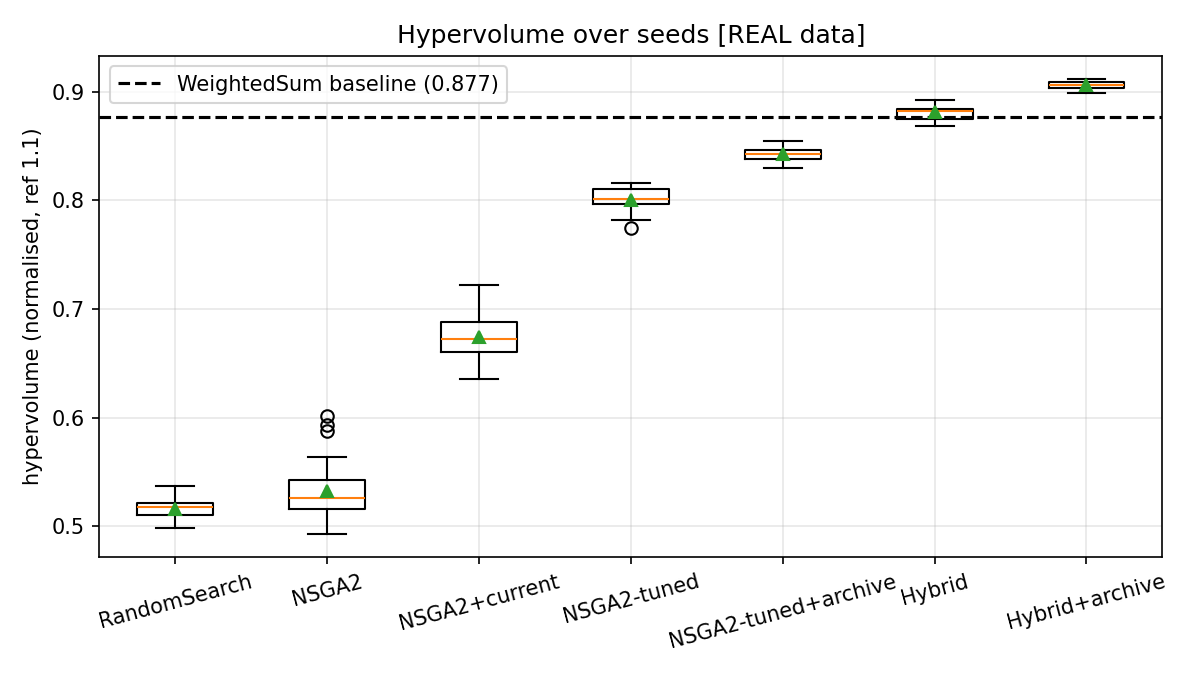
\includegraphics[width=.95\linewidth]{images/optimization_results.png}
\caption{Distribution of hypervolume across the recorded seeds. Source: repository real-data figure.}
\end{figure}
The final method improves mean HV by $(0.90659/0.87705-1)\times100=3.37\%$ and reduces mean IGD by approximately 62.4\% relative to the weighted-sum baseline. Its mean runtime is 7.74 times higher. Both the final-method sign test and Wilcoxon calculation give $p=1.86\times10^{-9}$ across the 30 saved runs.

Plain NSGA-II improves only modestly over random search. Current-portfolio injection, the tuned support strategy and archiving each increase HV. Convex refinement is necessary to surpass the stronger baseline in this experiment. Sparse initialization and reset mutation are introduced together, so this comparison does not isolate their individual effects.

\newsec{Pareto Front and a Worked Portfolio Example}
\begin{figure}[H]\centering
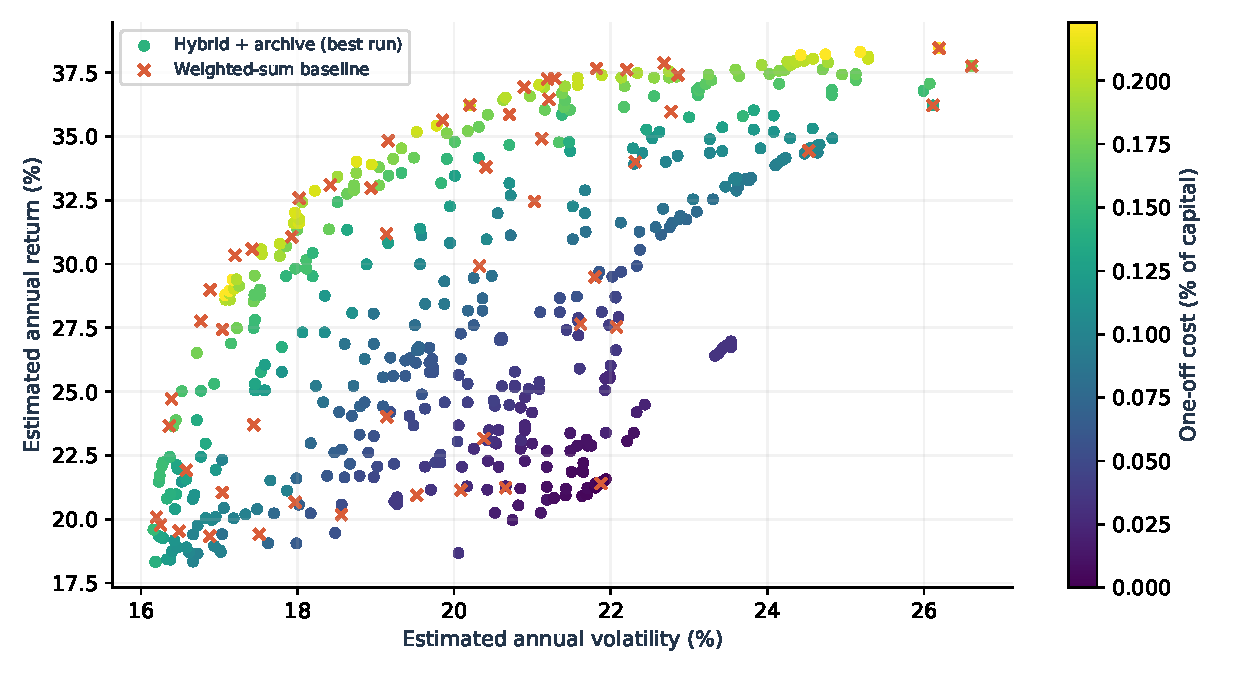
\includegraphics[width=.96\linewidth]{images/pareto_front.pdf}
\caption{Return--volatility projection of saved best-HV fronts. Color encodes the hybrid's one-off cost. These are representative best runs, not 30-seed means.}
\end{figure}
The saved Hybrid + archive best-run front contains 510 portfolios, spanning estimated annual returns of 18.33--38.46\%, volatility of 16.16--26.61\%, and one-off costs of approximately 0--0.223\% of capital. A two-dimensional projection cannot fully represent three-objective dominance: a higher-return, lower-volatility alternative may still cost more to enter.

The ``knee'' selector chooses the point closest to the ideal after independently min--max scaling the three front objectives. It is a balanced distance heuristic, not a curvature-based knee detector. Applied to the saved best-run front, it selects estimated return 31.12\%, volatility 19.58\% and one-off cost approximately 0.108\%.
\begin{table}[H]\centering\small
\begin{tabular}{@{}lrrlrr@{}}\toprule
Stock & Old \% & Target \% & Stock & Old \% & Target \%\\\midrule
TCS &20.00&20.00& CIPLA &0.00&6.93\\
RELIANCE &20.00&19.61& SBIN &15.00&6.53\\
ASIANPAINT &0.00&14.77& HDFCBANK &20.00&5.50\\
INFY &0.00&11.46& POWERGRID &0.00&5.05\\
WIPRO &0.00&7.15& TATASTEEL &0.00&3.00\\
ITC &15.00&0.00& LT &10.00&0.00\\\bottomrule
\end{tabular}
\caption{Rounded weights of the saved balanced example; small rounding differences may affect totals.}
\end{table}
For illustrative capital of INR 100,000, the modeled trading cost is about INR 108. This is a demonstration of the saved estimation-period solution, not a current-market recommendation. Its ten held stocks satisfy the configured position and sector limits.

\newsec{Out-of-Sample Walk-Forward Evaluation}
\subsection{Protocol}
At each rebalance row $t$, estimate inputs from rows $t-756$ through $t-1$, choose a target portfolio and deduct its trading cost. Hold for 63 trading days using actual subsequent price ratios. Portfolio weights drift as stocks grow at different rates; each strategy's drifted weights become its own next current portfolio. Fifteen complete periods cover 21 January 2022--20 November 2025. Remaining tail observations are not used for a partial period.

The stochastic strategies use five algorithmic paths on the same historical prices. These are not five independent market histories. ``NSGA-II'' here means the tuned, archived variant; ``Hybrid'' also includes archive and convex polish. Equal weight holds all 30 stocks and therefore does not obey the ten-stock limit. Do-nothing holds the initial shares, allowing weights to drift.
\begin{table}[H]\centering\small
\begin{tabular}{@{}lrrrr@{}}\toprule
Strategy & Wealth: knee & Wealth: ratio & CAGR: knee & Vol.: knee\\\midrule
Do nothing &1.6038&1.6038&13.43\%&14.27\%\\
Equal weight &\textbf{1.8428}&\textbf{1.8428}&17.70\%&12.77\%\\
Weighted sum &1.5641&1.5366&12.67\%&14.79\%\\
Tuned NSGA-II + archive &1.6298&1.5924&13.88\%&14.62\%\\
Hybrid + archive &1.5703&1.5505&12.78\%&14.59\%\\\bottomrule
\end{tabular}
\caption{Committed walk-forward summary values. Wealth starts near one after the initial trading-cost deduction; stochastic values are means across five paths.}
\end{table}
\begin{figure}[H]\centering
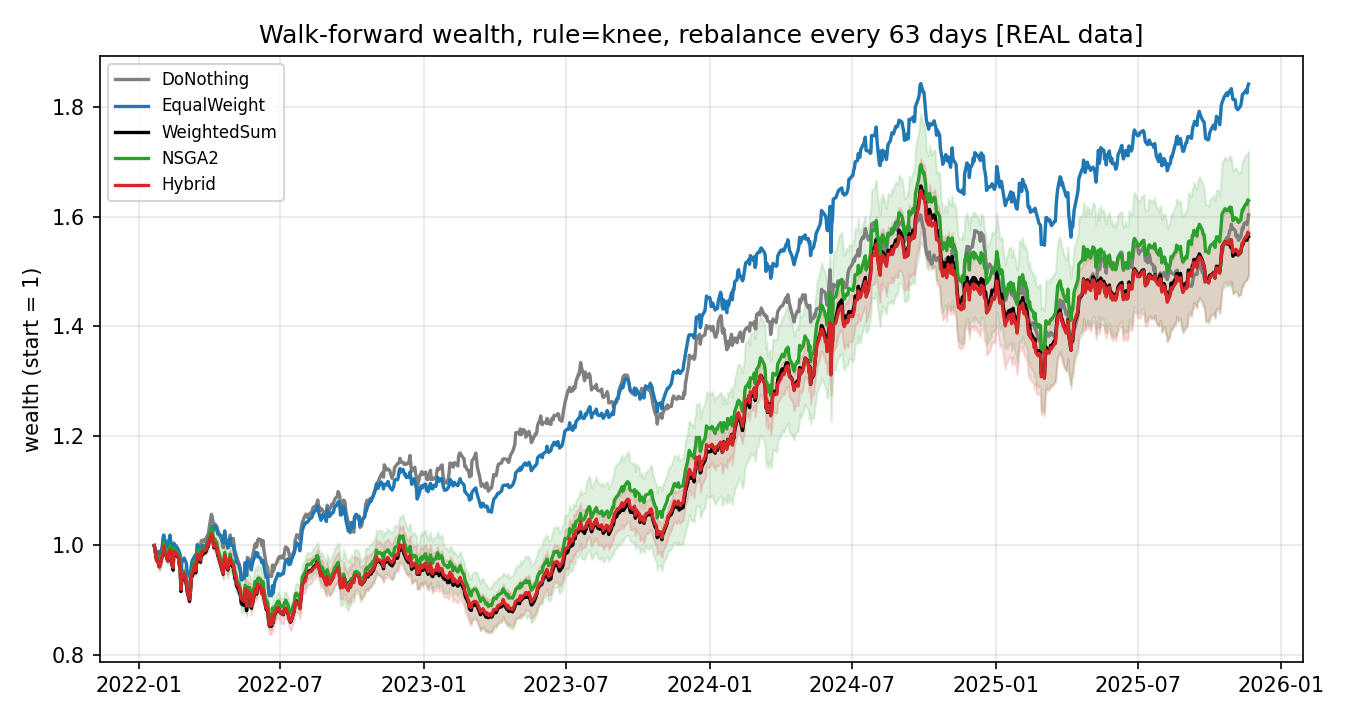
\includegraphics[width=.96\linewidth]{images/backtest_results.png}
\caption{Historical wealth under the balanced selection rule. Shaded ranges show algorithmic-path minima and maxima, not statistical confidence intervals.}
\end{figure}
The ratio selector maximizes $(\widehat r-4c)/\widehat\sigma$ for a 63-day holding horizon. It annualizes the one-off charge for comparison; it is not a risk-free-rate-adjusted Sharpe ratio. Neither selection rule produces an optimized strategy that exceeds equal weight's recorded final wealth.

\newsec{Interpreting Realised Performance}
\begin{figure}[H]\centering
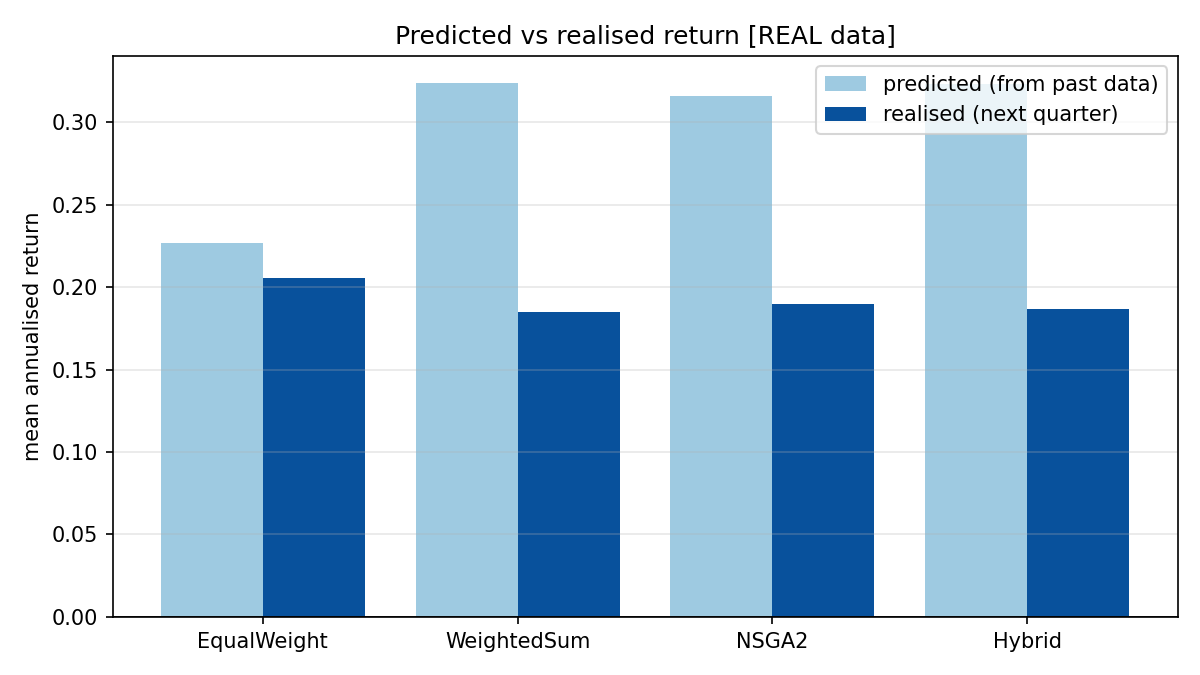
\includegraphics[width=.74\linewidth]{images/predicted_vs_realised.png}
\caption{Mean predicted annual return versus mean annualized subsequent-quarter return. These realised values are not the full-path CAGR. Source: repository real-data figure.}
\end{figure}
Under the balanced rule, Hybrid's mean predicted annual return is 32.29\%, while the mean annualized realised quarter return is 18.69\%. Its full-path CAGR is 12.78\%. These quantities differ because arithmetic estimates, individually annualized quarters and compounded multi-year returns are different measurements.
\subsection{Pairwise evidence}
Hybrid minus weighted sum averages approximately $+0.029$ percentage points per quarter, with reported standard error $0.101$ percentage points. The observed difference is too small relative to its uncertainty to support a reliable performance advantage. Hybrid minus equal weight averages $-0.940$ percentage points, with standard error $0.972$ percentage points. Only 15 periods are available, and serial dependence may make simple standard errors optimistic.
\subsection{Why front quality and wealth disagree}
The optimizer solves the estimated problem. It cannot correct an optimistic return vector merely by solving that problem more accurately. Sampling noise, regime changes and concentration affect realised outcomes. A broad 1/N benchmark uses fewer estimated inputs and more holdings, so its superior wealth is informative but not a like-for-like constrained optimum.
\note{\textbf{Practical interpretation.} The evidence supports improved coverage of the estimated return--risk--cost trade-off surface. It does not support a claim of market outperformance, superior forecasts or guaranteed investment gains.}
\subsection{Accounting detail}
The simulator deducts each rebalance charge before the subsequent holding period. Final wealth and its annualized growth therefore reflect trading costs. The separately reported mean annualized quarter return uses the post-cost starting capital for each quarter and excludes that quarter's entry charge. This difference in definitions must be retained when comparing the forecast chart with the net wealth table.

\newsec{Web Interface and Decision-Support Workflow}
The frontend branch adds a self-contained HTML/CSS/JavaScript page, a Python analysis engine and two server entry points. The local server uses Python's standard library and binds to \texttt{127.0.0.1}. For deployment, \texttt{app.py} exposes the same operations through Flask on Vercel. Both entry points reuse the shared application and optimization logic.

\textbf{Application URL:} \url{https://portfolio-pilot-deploy.vercel.app/}. The deployed application completed an example rebalance during verification on 14 November 2026. It is a decision-support interface and does not execute brokerage orders.
\subsection{User workflow}
\begin{enumerate}
\item Enter or edit current holdings and the capital amount; review the selected price source.
\item Request a rebalance. The engine freezes a price snapshot and estimates inputs from the latest 756 rows available in that snapshot.
\item Run tuned NSGA-II with archive and convex polish using a fixed seed.
\item Filter near-trivial options where possible, then select three to six representative portfolios.
\item Compare risk, expected return, trading cost, concentration and stock-level buy/sell amounts.
\item Consult the evidence and limitations views, which read the project's recorded experiment outputs.
\end{enumerate}
\subsection{Representative option selection}
The selection routine includes the lowest-volatility candidate, highest-return candidate and balanced ideal-distance point, then adds candidates farthest from those already selected in normalized objective space. It orders the resulting options by volatility. Filtering uses turnover and estimated improvement thresholds, with fallback when too few points remain.

This display layer intentionally reduces the full three-objective set. Its additional return--risk screening can hide portfolios that remain relevant because of cost; the selected options should therefore be described as a presentation subset, not the complete Pareto front.
\begin{table}[H]\centering\small
\begin{tabularx}{\linewidth}{@{}p{50mm}Y@{}}\toprule
API route & Purpose\\\midrule
\texttt{GET /api/context} & Universe, holdings defaults and available data-source information.\\
\texttt{GET /api/evidence} & Recorded optimizer and walk-forward summary results.\\
\texttt{POST /api/rebalance} & Validate holdings and return cached or newly optimized options.\\
\texttt{POST /api/refresh} & Download and cache a refreshed Yahoo Finance snapshot.\\\bottomrule
\end{tabularx}
\caption{API endpoints shared by the local server and the deployed Flask adapter.}
\end{table}
\subsection{Deployed example and result presentation}
\begin{figure}[H]\centering
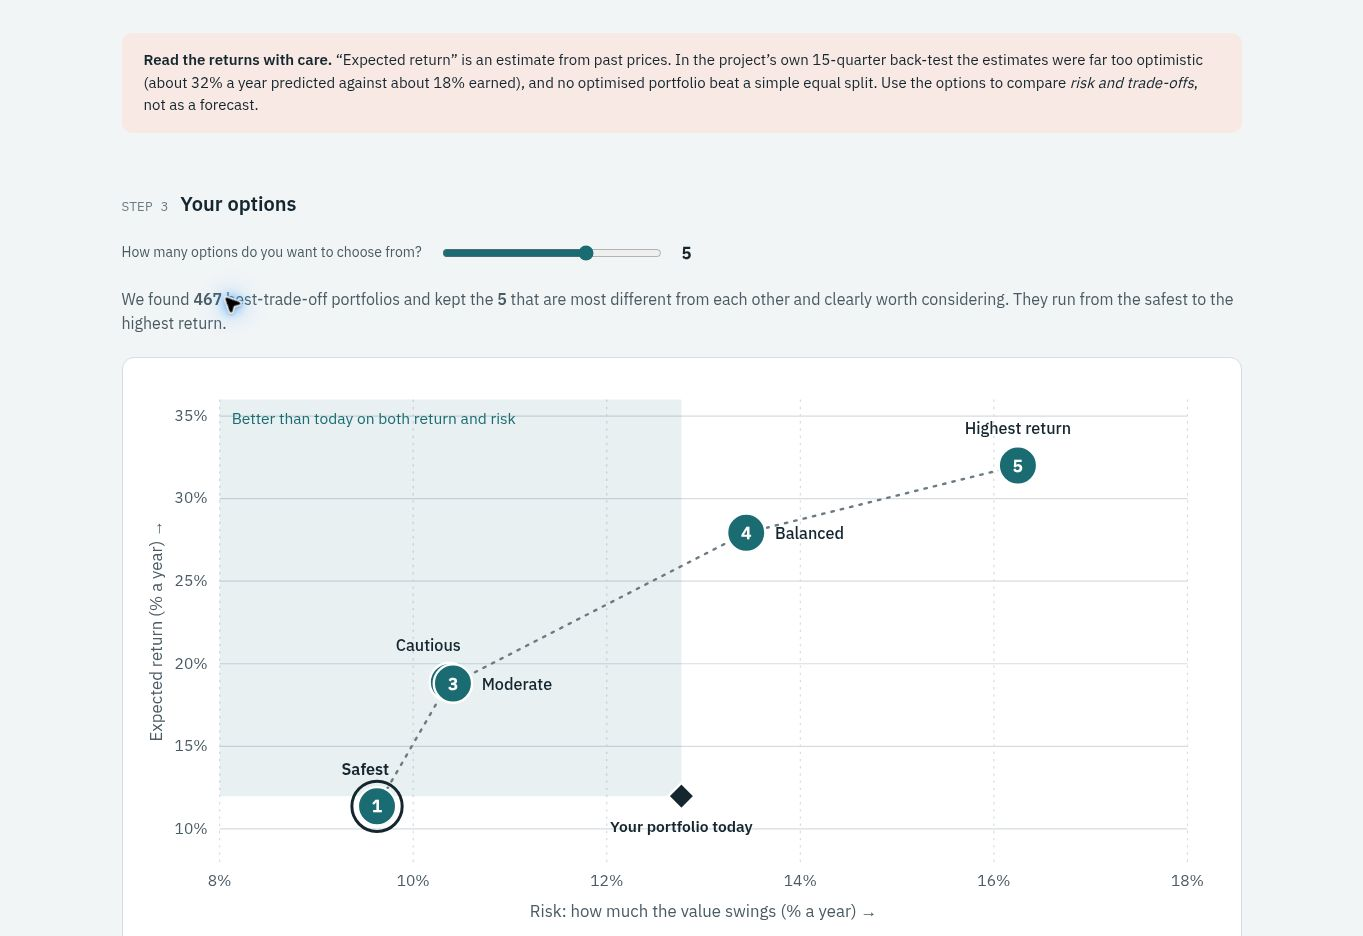
\includegraphics[width=.94\linewidth]{images/frontend_comparison.jpg}
\caption{Actual deployed application using the default hypothetical holdings and INR 1,000,000. This demonstration returned 467 trade-off portfolios and displayed five alternatives. The prices are a frozen snapshot ending 30 December 2025; displayed expectations are estimates, not realised results.}
\label{fig:frontend}
\end{figure}
The screenshot in Figure~\ref{fig:frontend} shows the current portfolio alongside the selected alternatives. Its values differ from the static experiment because the interface estimates from the latest window in the bundled data, whereas the static study uses the first window. The number of returned points is specific to this example and is not a fixed output-size guarantee.

\subsection{Deployment design}
The deployment requirements use \texttt{cvxpy-base} with the explicit CLARABEL solver to reduce unnecessary solver dependencies. The full research requirements remain in \path{requirements-project.txt}. The Vercel function configuration excludes reports, presentations, tests, figures and other non-runtime files from the function bundle. Temporary refreshed prices use \path{/tmp/portfoliopilot} in the hosted environment. Such cache contents are temporary and are not a persistent market-data store.

The Flask adapter limits request size, validates JSON input, returns structured errors and prevents stale browser responses with a no-store cache policy. A bounded in-memory result cache avoids repeating identical computations within a running instance. The web deployment is separate from the recorded experiment pipeline: deploying the interface does not regenerate or improve the saved research results.

\subsection{Reliability and communication}
The server validates numeric holdings, serializes optimization work and caches repeated input combinations. The committed data supports use without a fresh download. Explanation text is computed from portfolio outputs rather than generated by a language model. Terms such as ``safest'' mean lowest modeled volatility among displayed options; they do not establish bounded losses. The frontend's heuristic downside and payback statements should be replaced by calibrated uncertainty measures in a future version.

\newsec{Validation, Testing and Reproducibility}
\subsection{Convex-reference validation}
Removing cardinality and minimum-position rules creates a convex special case. The reference generator solves variance minimization over a $40\times12$ grid of return thresholds and cost ceilings, then filters the solutions. The committed reference contains 333 points. Across ten tuned evolutionary runs, mean HV relative to that reference is 0.86639, and mean IGD is 0.10469.

Although the module is named \texttt{exact\_front}, this is a finite solver-generated reference: individual convex subproblems are solved numerically, and a finite grid does not enumerate the entire continuous Pareto front. It validates approximate search behavior on a simpler model, not global optimality for the cardinality-constrained problem.
\subsection{Automated checks}
\begin{table}[H]\centering\small
\begin{tabularx}{\linewidth}{@{}p{42mm}Y@{}}\toprule
Area & Representative checks\\\midrule
Financial calculations & Return, covariance-based volatility, asymmetric transaction costs.\\
Feasibility and repair & Budget, cardinality, weight bounds, sector caps and adversarial key vectors.\\
Pareto and indicators & Dominance, sorting, crowding, hypervolume and related metrics.\\
Algorithms & Feasible non-dominated outputs, same-seed repeatability and archive cap.\\
Walk-forward & Schedule, drift arithmetic, portfolio selection and no-look-ahead estimation.\\
Frontend & Option selection, explanation payloads, input validation and local server behavior.\\\bottomrule
\end{tabularx}
\caption{Test responsibilities in the core and frontend branches.}
\end{table}
A verification run during preparation of the project materials completed \textbf{49 tests} on the frontend branch, covering the core and interface checks. Three CVXPY solution-accuracy warnings were emitted. Passing tests provide supporting evidence of implemented behavior, not a proof that every numerical solver result is exact.
\subsection{Evidence boundaries}
The headline CSV tables, selected portfolio weights, initial price-window dates and significance calculation were checked directly during report preparation. The tables report the committed experiment outputs rather than a new run of the full experiment pipeline. Recorded runtimes therefore remain original measurements. Package requirements use lower bounds rather than a fully locked environment; future reproduction should record exact versions and hardware.
\subsection{Suggested verification sequence}
Start with the unit tests, inspect the committed result files, reproduce the static experiment, and finally reproduce both rolling selection rules. Explicitly pass \texttt{--source real}; the configuration file's default data source is synthetic. Appendix~\ref{app:reproduce} provides the commands and output locations.

\newsec{Limitations and Future Scope}\label{sec:future}
\subsection{Limitations of the current study}
\begin{itemize}
\item \textbf{Estimation risk:} expected returns are historical sample means, without shrinkage, a factor forecast or robust uncertainty sets.
\item \textbf{Dataset scope:} one fixed universe and one historical market path limit external validity. Thirty random seeds measure optimizer variability, not market uncertainty.
\item \textbf{Cost and execution model:} simplified proportional charges omit fixed fees, spread, market impact, tax-on-gains and integer share quantities.
\item \textbf{Benchmark comparability:} equal weight holds 30 stocks; the optimization model permits ten. A constrained equal-weight benchmark is needed for tighter comparisons.
\item \textbf{Computational fairness:} the hybrid's extra solves and larger front improve quality at additional runtime. A matched-time experiment has not been established.
\item \textbf{Development bias:} tuning used the initial estimation problem; separate final seeds do not make this an untouched problem-level test set.
\item \textbf{Validation and numerics:} finite-grid convex validation and unit tests do not prove global optimality or correctness for all possible configurations.
\end{itemize}
\subsection{Proposed extensions, not implemented results}
\begin{table}[H]\centering\small
\begin{tabularx}{\linewidth}{@{}p{38mm}YY@{}}\toprule
Proposed idea & Intended benefit & Evaluation plan\\\midrule
Return shrinkage / factor estimates & Reduce optimistic and unstable means. & Repeat walk-forward with identical costs and constraints.\\
Robust optimization & Incorporate uncertainty in estimated returns. & Vary uncertainty budgets and measure net wealth and turnover.\\
Adaptive rebalance threshold & Avoid trades whose estimated benefit is too small. & Compare fixed quarterly and threshold-based schedules.\\
Stock-specific costs and lot sizes & Improve execution realism. & Add fees, spreads and integer shares; report feasibility and residual cash.\\
Matched-time and constrained benchmarks & Separate algorithm quality from compute and diversification. & Match runtimes; add ten-stock equal weight and a small exact mixed-integer case.\\
Uncertainty-aware interface & Replace point-estimate confidence with measured ranges. & Add scenario intervals and assess explanation comprehension.\\\bottomrule
\end{tabularx}
\caption{Future development ideas and how their value should be tested.}
\end{table}

\newsec{Conclusion and Project Contributions}
PortfolioPilot implements a complete constrained multi-objective portfolio rebalancing workflow: data estimation, feasibility repair, evolutionary search, solver-assisted refinement, comparative evaluation and decision-support presentation. Its central design insight is to use evolutionary search for stock selection and convex optimization for allocation within each selected support.

On the saved real-data experiment, Hybrid + archive reaches mean hypervolume 0.90659 and exceeds the weighted-sum baseline in all 30 seeds. The gain is approximately 3.37\%, with a recorded runtime increase of 7.74 times. Plain evolutionary search does not surpass the strong solver-based baseline, making the hybrid contribution and its computational cost explicit.

The walk-forward study provides a necessary counterpoint. Neither optimized strategy surpasses the equal-weight wealth benchmark. The final method is consequently best understood as a tool for exploring feasible estimated trade-offs, rather than evidence that historical-return optimization consistently generates superior investment outcomes.
\subsection{Individual contributions}
\begin{table}[H]\centering
\begin{tabularx}{\linewidth}{@{}p{30mm}Y@{}}\toprule
Member & Responsibilities recorded in the repository\\\midrule
Akhil\newline 241070004 & Topic selection and formulation; repository structure; data loader; problem model and repair; NSGA-II; random-search and weighted-sum baselines; metrics; unit tests; mid-evaluation preparation; final-report review and slides.\\
Ridhima\newline 241071062 & Real-data download and data documentation; cost assumptions; 30-seed real-data experiments; archive and hybrid runs; walk-forward evaluation; final results and documentation; fresh-clone verification.\\\bottomrule
\end{tabularx}
\caption{Contribution summary based on \texttt{report/contributions.md}; no new individual attribution is inferred for the frontend.}
\end{table}
\subsection{Development milestones}
The recorded development sequence progresses from formulation and core implementation to real-data experiments, archive and hybrid evaluation, walk-forward testing, interface development and final documentation.

\clearpage\appendix
\section{Reproduction and Report Build Guide}\label{app:reproduce}
\subsection{Environment and core experiment}
The repository specifies Python 3.9 or newer. Run from the project root:
\begin{lstlisting}
python3 -m venv .venv
source .venv/bin/activate
pip install -r requirements.txt
python -m pytest -q tests
python main.py experiment --source real --tag real
python main.py walkforward --source real --tag real --rule knee
python main.py walkforward --source real --tag real --rule ratio
python main.py figures --tag real
python main.py inspect --tag real --method Hybrid+archive --pick knee
\end{lstlisting}
The experiment regenerates outputs in the specified tag directory. Use another tag when preserving the committed results is important. For the frontend branch, install \path{requirements-project.txt} for tests and research commands, or \texttt{requirements.txt} for the hosted application dependencies. The local interface runs through \texttt{python main.py serve}. The hosted adapter is \texttt{app.py}.
\subsection{Evidence map}
\begin{table}[H]\centering\small
\begin{tabularx}{\linewidth}{@{}p{49mm}Y@{}}\toprule
Report content & Repository source\\\midrule
Configuration and universe & \texttt{config/default.json}, \texttt{config/universe.csv}\\
Price snapshot and assumptions & \texttt{data/prices\_real.csv}, \texttt{data/DATA.md}\\
Static metrics and statistics & \texttt{results/real/summary.csv}, \texttt{per\_seed\_metrics.csv}, \texttt{stats.json}\\
Illustrative allocation & \texttt{results/real/best\_front\_Hybrid\_archive.csv}\\
Rolling results & \texttt{results/real/walkforward\_knee/} and \texttt{walkforward\_ratio/}\\
Convex validation & \texttt{results/real/validation\_convex.json}\\
Interface implementation & \texttt{frontend/engine.py}, \texttt{server.py}, \texttt{static/index.html} on frontend branch\\\bottomrule
\end{tabularx}
\caption{Sources of the principal report claims. Relative filenames in the static-metrics row share the same directory.}
\end{table}
\subsection{Compile this report}
The source bundle is self-contained. With a standard TeX Live installation, run twice from its directory:
\begin{lstlisting}
pdflatex -interaction=nonstopmode -halt-on-error PortfolioPilot_Report.tex
pdflatex -interaction=nonstopmode -halt-on-error PortfolioPilot_Report.tex
\end{lstlisting}
The second pass resolves contents, citations and cross-references. Assets are included locally; no live data download is required to rebuild the document.

\newsec{Stock Universe}\label{app:universe}
\begin{table}[H]\centering\small
\begin{tabularx}{\linewidth}{@{}p{34mm}Y@{}}\toprule
Sector & NSE tickers (each uses the Yahoo Finance suffix \texttt{.NS})\\\midrule
Financials & HDFCBANK, ICICIBANK, SBIN, KOTAKBANK, AXISBANK\\
Information technology & TCS, INFY, WIPRO, HCLTECH\\
FMCG & HINDUNILVR, ITC, NESTLEIND, BRITANNIA\\
Energy / Power & RELIANCE, ONGC, NTPC, POWERGRID, COALINDIA\\
Automobiles & MARUTI, M\&M, EICHERMOT\\
Pharmaceuticals & SUNPHARMA, DRREDDY, CIPLA\\
Materials & TATASTEEL, HINDALCO, ULTRACEMCO, ASIANPAINT\\
Infrastructure / Telecom & LT, BHARTIARTL\\\bottomrule
\end{tabularx}
\caption{Universe as configured in \texttt{config/universe.csv}. Sector labels follow the project taxonomy.}
\end{table}
\subsection{Notation and abbreviations}
\begin{table}[H]\centering
\begin{tabularx}{\linewidth}{@{}p{34mm}Y@{}}\toprule
Symbol / term & Meaning\\\midrule
$x$, $x^{old}$ & Target and current portfolio-weight vectors.\\
$\mu$, $\Sigma$ & Estimated annual return vector and covariance matrix.\\
$H$, $K$ & Held-stock support; maximum permitted holdings.\\
$b_i$, $s_i$ & Buy and sell cost rates for stock $i$.\\
HV & Hypervolume; larger indicates better dominated coverage for fixed scaling.\\
IGD & Inverted generational distance; smaller indicates closer reference coverage.\\
SBX & Simulated binary crossover.\\
CAGR & Compound annual growth rate.\\
NSGA-II & Non-dominated Sorting Genetic Algorithm II.\\
Archive & Bounded store of feasible non-dominated discoveries.\\\bottomrule
\end{tabularx}
\caption{Notation used in the report.}
\end{table}
\note{\textbf{Reading percentages.} A return of 0.31 means 31\% annually; a cost of 0.00108 means 0.108\% once. A return change from 20\% to 25\% is five percentage points, not a five-percent relative increase.}

\clearpage
\addcontentsline{toc}{section}{References}
\begin{thebibliography}{99}\small\emergencystretch=2em
\bibitem{markowitz} H. Markowitz, ``Portfolio Selection,'' \emph{The Journal of Finance}, vol. 7, no. 1, pp. 77--91, 1952.
\bibitem{deb} K. Deb, A. Pratap, S. Agarwal, and T. Meyarivan, ``A fast and elitist multiobjective genetic algorithm: NSGA-II,'' \emph{IEEE Transactions on Evolutionary Computation}, vol. 6, no. 2, pp. 182--197, 2002. \url{https://doi.org/10.1109/4235.996017}.
\bibitem{chang} T.-J. Chang, N. Meade, J. E. Beasley, and Y. M. Sharaiha, ``Heuristics for cardinality constrained portfolio optimisation,'' \emph{Computers \& Operations Research}, vol. 27, no. 13, pp. 1271--1302, 2000.
\bibitem{lobo} M. S. Lobo, M. Fazel, and S. Boyd, ``Portfolio optimization with linear and fixed transaction costs,'' \emph{Annals of Operations Research}, vol. 152, pp. 341--365, 2007. \url{https://web.stanford.edu/~boyd/papers/portfolio.html}.
\bibitem{ledoit} O. Ledoit and M. Wolf, ``A well-conditioned estimator for large-dimensional covariance matrices,'' \emph{Journal of Multivariate Analysis}, vol. 88, no. 2, pp. 365--411, 2004.
\bibitem{demiguel} V. DeMiguel, L. Garlappi, and R. Uppal, ``Optimal versus naive diversification: How inefficient is the 1/N portfolio strategy?'' \emph{The Review of Financial Studies}, vol. 22, no. 5, pp. 1915--1953, 2009.
\bibitem{cvxpy} S. Diamond and S. Boyd, ``CVXPY: A Python-Embedded Modeling Language for Convex Optimization,'' \emph{Journal of Machine Learning Research}, vol. 17, no. 83, pp. 1--5, 2016. \url{https://www.jmlr.org/papers/v17/15-408.html}.
\bibitem{zitzler} E. Zitzler and L. Thiele, ``Multiobjective evolutionary algorithms: A comparative case study and the strength Pareto approach,'' \emph{IEEE Transactions on Evolutionary Computation}, vol. 3, no. 4, pp. 257--271, 1999.
\bibitem{sklearn} F. Pedregosa et al., ``Scikit-learn: Machine Learning in Python,'' \emph{Journal of Machine Learning Research}, vol. 12, pp. 2825--2830, 2011.
\bibitem{repo} Akhil and Ridhima, \emph{PortfolioPilot: source code, data and experimental outputs}, 2026. \url{https://github.com/akhil-gitcoder/PortfolioPilot}. Inspected 14 November 2026; core commit \texttt{482fe84}, frontend commit \texttt{96aa4d5}.
\end{thebibliography}
\end{document}
